\documentclass{beamer}

\usepackage[english]{babel}
\usepackage{xcolor}
\usepackage{xmpmulti}
\usepackage{amsmath}
\usepackage{dsfont}
\usepackage{multicol}
\usepackage{tikz}
\usepackage{eucal}
\usetikzlibrary{positioning,angles,quotes}
\usepackage{url}
\usepackage{graphicx}
\usepackage{cmbright}
\usepackage{framed}
\usepackage{tabularx}
\usepackage{amssymb}
\usepackage{pifont}


\usetikzlibrary{pgfplots.groupplots,arrows.meta,shadows,positioning,angles,quotes}
\usetikzlibrary{matrix,chains,positioning,decorations.pathreplacing,arrows}
\usepackage{tikz}
\usetikzlibrary{shapes.geometric}
\usetikzlibrary{positioning}
\usepackage{pgfplots}

%\input{epgfplotslibrary{groupplots}
\usetikzlibrary{pgfplots.groupplots,arrows.meta,shadows,positioning,angles,quotes}
\usetikzlibrary{matrix,chains,positioning,decorations.pathreplacing,arrows}

\newcommand{\xmark}{\ding{55}}

\DeclareMathOperator*{\argmax}{arg\,max}
\def\checkmark{\tikz\fill[scale=0.4](0,.35) -- (.25,0) -- (1,.7) -- (.25,.15) -- cycle;} 

\definecolor{Maroon}{cmyk}{0, 0.87, 0.68, 0.32}
\definecolor{RoyalBlue}{cmyk}{1, 0.50, 0, 0}
\definecolor{skymagenta}{rgb}{0.81, 0.44, 0.69}

\newenvironment{takeaway}[1]{%
	\definecolor{shadecolor}{gray}{0.9}%
		\begin{shaded}{\color{skymagenta}\noindent\textsc{#1}}\\%
		}{%
		\end{shaded}%
}



%%%%%% THE FOLLOWING FILE CONTAINS THE STYLE DEFINITIONS %%%%%%
\usepackage[utf8]{inputenc}
\usepackage[export]{adjustbox}

\definecolor{gris}{rgb}{0.92,0.92,0.92}
\definecolor{blau-upc}{rgb}{.192,.365,.506}

\setbeamercolor{titlelike}{fg=blau-upc}
% \setbeamercolor{barra}{bg=white,fg=white}
\setbeamercolor{capcalera}{bg=blau-upc,fg=white}
\setbeamercolor{section in toc}{fg=blau-upc}
\setbeamertemplate{sections/subsections in toc}[circle]
\setbeamertemplate{itemize items}[circle]
\setbeamercolor{item}{fg=blau-upc}
\setbeamertemplate{blocks}[rounded][shadow=true]
\setbeamercolor*{block body}{bg=gris}
\setbeamerfont{block body}{size=\footnotesize}
\setbeamercolor*{block title}{parent=structure,bg=blau-upc,fg=white}

\setbeamersize{text margin left=12mm,text margin right=12mm}
\setbeamertemplate{navigation symbols}{}

\setbeamertemplate{footline}[frame number]{}


\defbeamertemplate*{headline}{infolines theme}
{
	\begin{beamercolorbox}[wd=\paperwidth,ht=6.5mm,right]{white}%
		%\includegraphics[width = 45mm, height=10mm]{./logotips/visapp}\hspace*{2mm}\vskip0.2ex
	\end{beamercolorbox}
 	\begin{beamercolorbox}[wd=\paperwidth,ht=0.5mm,left]{barra}%
 		\hspace*{1mm}
 	\end{beamercolorbox}
}

\setbeamertemplate{footline}
{
	\hbox{
	\begin{beamercolorbox}[wd=0.1\paperwidth,ht=10mm,left]{}
% 		\hspace*{1ex}\includegraphics[height=8mm]{./logotips/imperiallogo.pdf}\vskip 2ex
	\end{beamercolorbox}
	\begin{beamercolorbox}[wd=0.8\paperwidth,ht=3ex,center]{}
		\hspace*{4ex}\insertsection\vskip 4ex
	\end{beamercolorbox}
	\begin{beamercolorbox}[wd=0.1\paperwidth,ht=3ex,right]{}
		\insertpagenumber\hspace*{6ex}\vskip 4ex
	\end{beamercolorbox}
	}
}

\setbeamertemplate{title page}
{
	\vbox{}
	\vfill
	\begin{centering}
		{\usebeamerfont{title}\usebeamercolor[fg]{title}\inserttitle}
		\vskip0.2em
		{\usebeamerfont{subtitle}\usebeamercolor[fg]{subtitle}\insertsubtitle}
		\vskip2em\par
		\small\insertauthor\par
		\vskip2em\par
		\tiny\insertdate\vskip1em\par
	\end{centering}
% 	\vfill
}

%\usebackgroundtemplate{\put(-50,-340){\includegraphics[width=10cm]{}}} 

%%%%%%

%%%%%% TITLE, AUTHOR, DATE DEFINITIONS %%%%%%
\title{Function Approximators}
\subtitle{Scaling Reinforcement Learning Algorithms to High-Dimensional Problems}
\author{Matthia Sabatelli}

\date{\today}
%%%%%%

\setbeamertemplate{footline}[frame number]{}

\begin{document}

\frame{\titlepage} 

\begin{frame}{Recap}

	Last week we have seen ...
	\begin{block}{Model-Free Reinforcement Learning}
		\begin{itemize}
			\item How to construct algorithms when parts of the MDP $\mathcal{M}$ are unknown
			\item Monte-Carlo (MC) Learning
			\item Temporal-Difference (TD) Learning
			\item The concept of bootstrapping
			\item How to learn $Q^{\pi}(s,a)$ in an \textit{on-policy} fashion or in an \textit{off-policy} fashion
		\end{itemize}
	\end{block}

\end{frame}


\frame{\frametitle{Today's Agenda}\tableofcontents}


\begin{frame}{Function Approximation}
	\section{Function Approximation}

	The algorithms that we have seen last week are typically implemented in a \textcolor{RoyalBlue}{tabular} fashion:
	\begin{itemize}
		\item If the goal is to learn $V^{\pi}(s)$ we use a table of size $|\mathcal{S}|$
		\item If the goal is to learn $Q^{\pi}(s,a)$ we use a table of size $|\mathcal{S}\times\mathcal{A}|$
	\end{itemize}

	It is easy to see the \textcolor{Maroon}{limitations} of this approach:

	\begin{enumerate}
		\item Unfeasible when the state-action space is large
		\item Impossible to use in a continous setting
		\item Requires a discretization of the environment
		\item Lacks generalization
	\end{enumerate}

\end{frame}


\begin{frame}{Function Approximation}
	A simple example: the game of Go
	\bigskip

	\begin{center}
		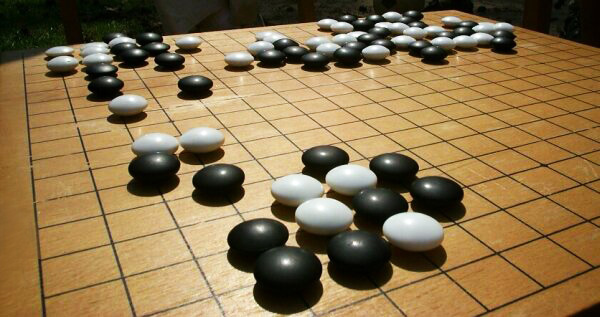
\includegraphics[width=\textwidth]{./Images/Go_board}
	\end{center}

\end{frame}

\begin{frame}{Function Approximation}

	A simple \textcolor{RoyalBlue}{example}: the game of Go
	
	\begin{itemize}
		\item The AlphaGo and AlphaZero programs are a typical example of the recent success of Reinforcement Learning
		\item Both programs heavily rely on a \textcolor{RoyalBlue}{function approximator}
	\end{itemize}
	
	\bigskip

	\textcolor{Maroon}{Why?}

	\begin{itemize}
		\item The size of the Go board is $19\times19$
		\item On each location there can, or can't, be a stone (white or black)
		\item State space $|\mathcal{S}| = 3^{19\times19}=3^{361}$
	\end{itemize}

	\bigskip
	
	\centering
	\textcolor{Maroon}{Impossible to learn any value function!}

\end{frame}

\begin{frame}{Function Approximation}
	Another \textcolor{RoyalBlue}{example}: the Atari-2600 benchmark
	\bigskip

	\begin{center}
		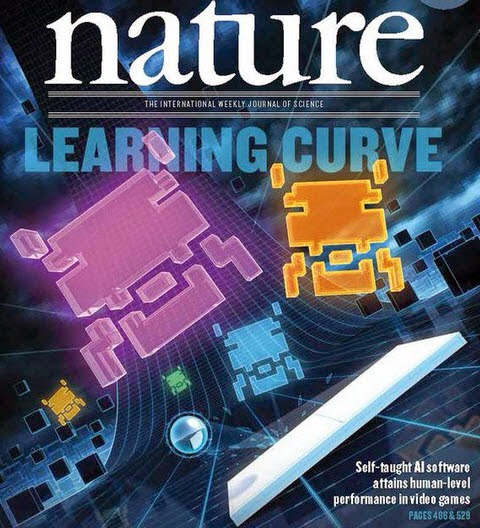
\includegraphics[width=5cm]{./Images/nature}
	\end{center}

\end{frame}

\begin{frame}{Function Approximation}
	Another \textcolor{RoyalBlue}{example}: the Atari-2600 benchmark

	\begin{itemize}
		\item The first Deep Reinforcement Learning agent of mastering these games is based on a \textcolor{RoyalBlue}{Convolutional Neural Network}
		\item The network was trained on the raw input pixels of the game
	\end{itemize}
	
	\begin{center}
		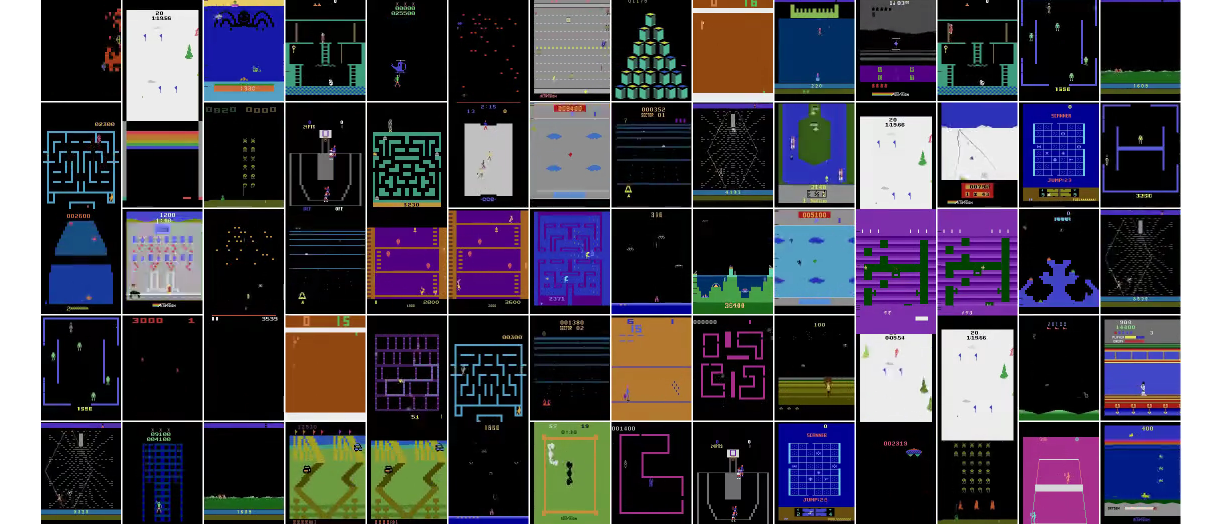
\includegraphics[width=8cm]{./Images/games}
	\end{center}
\end{frame}


\begin{frame}{Function Approximation}
	Let's take a look at some states of the \texttt{Pong} game:
	\begin{center}
		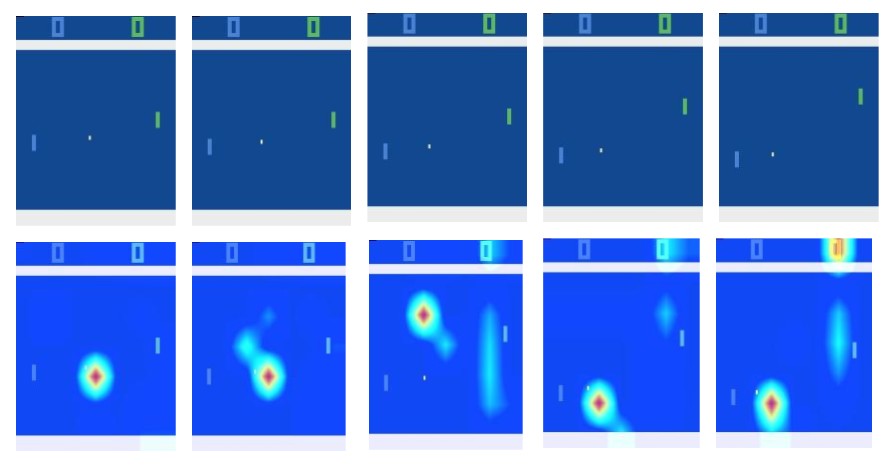
\includegraphics[width=8cm]{./Images/pong}
	\end{center}


	\begin{itemize}
		\item All states look very \textcolor{RoyalBlue}{similar} among each other
		\item Small portions of the state-space are actually \textcolor{RoyalBlue}{informative}
		\item Despite some pre-processing operations the state-space stays \textcolor{RoyalBlue}{highly dimensional}
	\end{itemize}

\end{frame}


\begin{frame}{Function Approximation}
	Fortunately we can \textcolor{RoyalBlue}{overcome} the aforementioned \textcolor{Maroon}{issues} by including a function approximator in the reinforcement learning cooking recipe!
	\begin{block}{Function Approximators}
		We \textcolor{Maroon}{do not} represent a value function as a table anymore, but rather with a \textcolor{RoyalBlue}{parametrized functional form} with weight vector $\mathbf{w}\in\mathds{R}^{d}$.


		Therefore we are now interested in learning:
		\begin{align*}
			V^{\pi}(s) \approx \hat{V}^{\pi}(s;\mathbf{w})
		\end{align*}
	\end{block}

\end{frame}

\begin{frame}{Function Approximation}

	We will see that $\hat{V}(s;\mathbf{w})$ can come in numerous forms but the \textcolor{Maroon}{key} ideas behind using a function approximator are always the same:
	\begin{enumerate}
		\item We want to \textcolor{RoyalBlue}{overcome} the computational burdens that come from large state $|\mathcal{S}|$ and action $|\mathcal{A}|$ spaces
		\item We wish to \textcolor{RoyalBlue}{represent} states through informative features
		\item Ideally we would like to learn an approximation of a value function which \textcolor{RoyalBlue}{generalizes} well across states
	\end{enumerate}

	\bigskip

	$\Rightarrow$ Now that we have built some intuition around why function approximation is useful let us dive deeper into this family of techniques ...


\end{frame}

\begin{frame}{Linear Functions}
	\section{Linear Functions}

	Any function approximator comes is the following form:
	\begin{align*}
		y = f(\mathbf{x};\mathbf{w})
	\end{align*}


	The \textcolor{RoyalBlue}{easiest} form of a function approximator that we can use is a \textcolor{RoyalBlue}{linear} function 	which is linear in the components of $\mathbf{x}$:

	\bigskip

	For example we can represent the value of a state as a two-dimensional feature vector: 
	\begin{align*}
		\mathbf{x}=[f_1(s), f_2(s), ..., f_i(s)] \in \mathds{R}^2
	\end{align*}

\end{frame}


\begin{frame}{Linear Functions}
	\begin{takeaway}{Quiz Time!}
		Given the popular \texttt{Pacman} game, which features would you consider to be the most representative ones of the game?
	
	\end{takeaway}
	\begin{center}
		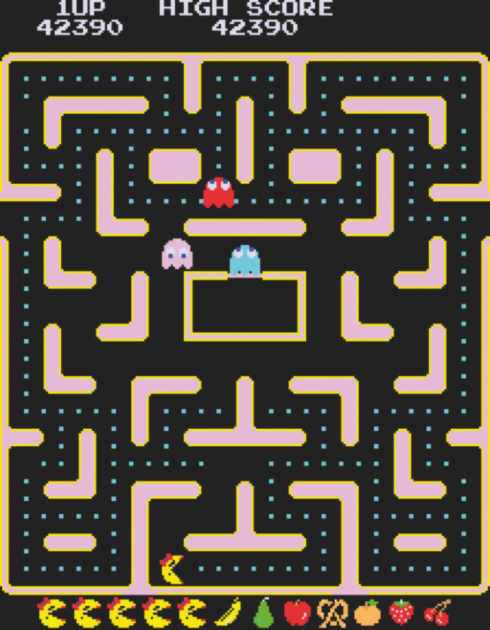
\includegraphics[width=4cm]{./Images/p}
	\end{center}

\end{frame}

\begin{frame}{Linear Functions}
	So far we have seen:
	\begin{enumerate}
		\item Why it is \textcolor{RoyalBlue}{desirable} to have a function approximator
		\item One of the possible \textcolor{RoyalBlue}{forms} of such function 
		\item How crucial it is to carefully go through a process of \textcolor{RoyalBlue}{feature engineering} 
	\end{enumerate}
	\bigskip

	\centering

	\textcolor{Maroon}{However ...}

	\bigskip
	\textit{How do we train these functions?}

\end{frame}

\begin{frame}{Linear Functions}
	\begin{center}
		We use \textcolor{RoyalBlue}{Stochastic Gradient Descent} (SGD):
	\end{center}
	
	\bigskip

	\begin{itemize}
		\item We have a weight vector $\mathbf{w}\doteq(w_1, w_2, ..., w_d)$ of real values parametrizing our function approximator
		\item The approximate value function $\approx \hat{V}^{\pi}(s;\mathbf{w})$ is a differentiable function of $\mathbf{w}$ for all $s\in\mathcal{S}$
		\item As SGD works in an iterative fashion we will make use of the underscript $t$ denoting $\mathbf{w}_t$
	\end{itemize}
\end{frame}


\begin{frame}{Linear Functions}
	A simple example:
	\begin{itemize}
		\item We wish to evaluate the state-value function $V^\pi(s)$
		\item We assume that the correct values of a state are \textcolor{RoyalBlue}{known} 
		\item We know the \textcolor{RoyalBlue}{true value} of a state under policy $\pi$
	\end{itemize}

	\begin{block}{SGD in practice}
		We wish to \textcolor{RoyalBlue}{minimize} the estimates made by $\hat{V}(s;\mathbf{w})$ with respect to $V^{\pi}(s)$:
		
		\begin{align*}
			\mathbf{w}_{t+1} & \doteq \mathbf{w}_t - \frac{1}{2} \alpha\nabla\Big[V^{\pi}(s_t)-\hat{V}(s;\mathbf{w}_t)\Big]^{2} \\ 
					 & = \mathbf{w}_t +\alpha\Big[V^{\pi}(s_t)-\hat{V}(s_t;\mathbf{w}_t)\Big]\nabla \hat{V}(s;\mathbf{w}_t)
		\end{align*}

		where $\alpha$ is the step-size and $\nabla f(\mathbf{w})$ is the vector containing all partial derivatives wrt to the components of $\mathbf{w}$:
		\begin{align*}
			\nabla f(\mathbf{w}) \doteq \Big(\frac{\partial f(\mathbf{w})}{\partial w_1}, \frac{\partial f(\mathbf{w})}{\partial w_2}, ..., \frac{\partial f(\mathbf{w})}{\partial w_d}\Big).
		\end{align*}

	\end{block}
\end{frame}

\begin{frame}{Linear Functions}
	So far ...
	\begin{itemize}
		\item We have considered the case where we have access to the \textcolor{RoyalBlue}{true value} of a state $V^{\pi}(s)$
		\item But in practice this is \textcolor{Maroon}{never the case} (see MC and TD-Learning)
		\item How to deal with the problem of \textcolor{RoyalBlue}{control}?
	\end{itemize}

	\bigskip 

	Let's see how to learn the state-action value function $\hat{Q}(s,a;\mathbf{w})$

\end{frame}

\begin{frame}{Linear Functions}
	We follow the same steps that we have used beforehand for learning $\hat{V}(s;\mathbf{w})$:
	\begin{enumerate}
		\item We take a model-free Reinforcement Learning algorithm of our choice
		\item We construct an objective function we wish to minimize 
		\item Perform gradient descent on the parameter vector $\mathbf{w}$
	\end{enumerate}


	\begin{block}{Q-Learning with function approximation}	
		\begin{align*}
			\uncover<+-> {Q(s_t,a_t) & :=Q(s_t,a_t) + \alpha\big[\underbrace{r_t + \gamma \:\underset{a\in \mathcal{A}}{\max}\:Q(s_{t+1},a_t)}_{y_t} - Q(s_t, a_t) \big].} \\
				\uncover<+-> {\mathcal{L} & = \frac{1}{2}\Big(y_t - Q(s_t, a_t)\Big)^2} \\
				\uncover<+-> {\frac{\partial \mathcal{L}}{\partial \mathbf{w}} & = - \Big(y_t -Q(s_t, a_t)\Big)\mathbf{x}(s_t)}
		\end{align*}

	\end{block}
	
\end{frame}

\begin{frame}{Linear Functions}

	Linear functions allow us to overcome the curse of dimensionality issue, but:
	\begin{enumerate}
		\item Their representational power is still \textcolor{Maroon}{limited}
		\item Require a \textcolor{Maroon}{careful} feature engineering stage
	\end{enumerate}

	\bigskip

	$\Rightarrow$ Therefore \textcolor{RoyalBlue}{non-linear} functions such as neural networks are preferred!
	\begin{itemize}
		\item They follow the same principles of linear functions 
		\item Are powerful feature extractors 
		\item Benefit from being universal function approximators
	\end{itemize}

	\bigskip

	\begin{center}
		Are \textcolor{Maroon}{\textbf{extremely hard and slow}} to train!
	\end{center}

\end{frame}


\begin{frame}{Neural Networks}
	\section{Neural Networks}

	\begin{center}
		\textcolor{skymagenta}{Welcome to the magical world of Deep Reinforcement Learning (DRL)!}
	\end{center}

	\begin{itemize}
		\item In DRL we use deep neural networks as \textcolor{RoyalBlue}{non-linear} function approximators
		\item However, if a single hidden layer network is used we talk about $\Rightarrow$ \textcolor{RoyalBlue}{Connectionist Reinforcement Learning}	
		\item But typically Convolutional Neural Networks are preferred $\Rightarrow$ \textcolor{RoyalBlue}{Deep Reinforcement Learning}
	\end{itemize}
	
\end{frame}

\begin{frame}{Neural Networks}

	Before AlphaGo and AlphaZero there was \textcolor{RoyalBlue}{TD-Gammon}:
	\begin{enumerate}
		\item The first computer program of mastering a boardgame  
		\item The first successful combination of Reinforcement Learning and neural networks
		\item The first practical application of TD-Learning
	\end{enumerate}

	\begin{center}
		$\Rightarrow$ Until $\approx 15$ years ago TD-Gammon was arguably the most (and only) successful application combining neural networks and Reinforcement Learning
	\end{center}
\end{frame}


\begin{frame}{Neural Networks}
	Some Reinforcement Learning history ...
	\bigskip

	\centering
		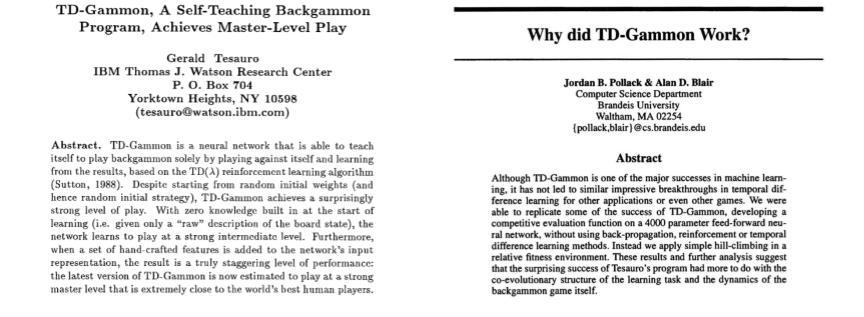
\includegraphics[width=11cm]{./Images/tdgammon}

\end{frame}

\begin{frame}{Neural Networks}
	But in $2013$ things started to change $\Rightarrow$ \textcolor{skymagenta}{Deep-Q Networks} (DQN) were introduced!

	\begin{enumerate}
		\item The community started to focus on using \textcolor{RoyalBlue}{Convolutional Neural Networks}
		\item Powerful networks able of serving as \textcolor{RoyalBlue}{function approximators} as well as \textcolor{RoyalBlue}{feature extractors}
		\item The first step was to adapt the Q-Learning algorithm 
	\end{enumerate}
	
	\bigskip 

	$\Rightarrow$ Let's see how DQN intuitively works!

\end{frame}


\begin{frame}{Neural Networks}

	\begin{figure}
		\centering
		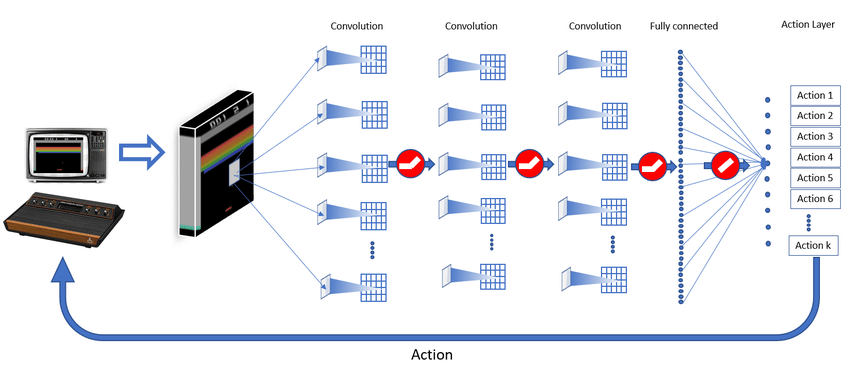
\includegraphics[width=10cm]{./Images/dqn}
		\caption{Image courtesy of Patel et al. (2019)}
	\end{figure}

\end{frame}

\begin{frame}{Neural Networks}
	\begin{center}
		How do we \textcolor{Maroon}{train} such a system?
		\begin{equation*}  
			Q(s,a;\theta)\approx Q^{*}(s,a)
		\end{equation*}
	\end{center}
\end{frame}



\begin{frame}{Neural Networks}
	\begin{center}
		How do we \textcolor{Maroon}{train} such a system?
		\begin{equation*}  
			Q(s,a; \textcolor{blue}{\theta})\approx Q^{*}(s,a)
		\end{equation*}
	\end{center}
\end{frame}



\begin{frame}{Neural Networks}
	\begin{center}
		How do we \textcolor{Maroon}{train} such a system?
		\begin{equation*}  
			Q(s,a; \textcolor{blue}{\theta})\approx Q^{*}(s,a)
		\end{equation*}
	\end{center}

	$\Rightarrow$ We reshape the Q-Learning algorithm into an \textcolor{RoyalBlue}{objective function} that can be used for learning $\theta$

	\begin{block}{The DQN Algorithm}
		
		\begin{equation*}
			Q(s_t,a_t):=Q(s_t,a_t) + \alpha\big[r_t + \gamma \:\underset{a\in \mathcal{A}}{\max} Q(s_{t+1},a_t) - Q(s_t, a_t) \big].
			\label{eq:q_learning}
		\end{equation*}
		\begin{multline*}
				\mathcal{L}(\theta) = \mathds{E}_{\langle s_{t},a_{t},r_{t},s_{t+1}\rangle\sim U(D)} \bigg[\big(r_{t} + \gamma \: \underset{a\in \mathcal{A}}{\max}\: Q(s_{t+1}, a; \theta^{-}) - Q(s_{t}, a_{t}; \theta)\big)^{2}\bigg].
		\end{multline*}
	\end{block}

\end{frame}


\begin{frame}{Neural Networks}
	\begin{center}
		How do we \textcolor{Maroon}{train} such a system?
		\begin{equation*}  
			Q(s,a; \textcolor{blue}{\theta})\approx Q^{*}(s,a)
		\end{equation*}
	\end{center}

	$\Rightarrow$ We reshape the Q-Learning algorithm into an \textcolor{RoyalBlue}{objective function} that can be used for learning $\theta$

	\begin{block}{The DQN Algorithm}
		
		\begin{equation*}
			Q(s_t,a_t):=Q(s_t,a_t) + \alpha\big[r_t + \gamma \:\underset{a\in \mathcal{A}}{\max} Q(s_{t+1},a_t) - Q(s_t, a_t) \big]
			\label{eq:q_learning}
		\end{equation*}
		\begin{multline*}
			\mathcal{L}(\theta) = \mathds{E}_{\langle s_{t},a_{t},r_{t},s_{t+1}\rangle\sim U(D)} \bigg[\textcolor{blue}{\big(}r_{t} + \gamma \: \underset{a\in \mathcal{A}}{\max}\: Q(s_{t+1}, a; \theta^{-}) - Q(s_{t}, a_{t}; \theta) \textcolor{blue}{\big)^{2}}\bigg]
		\end{multline*}
	\end{block}
\end{frame}



\begin{frame}{Neural Networks}
	\begin{center}
		How do we \textcolor{Maroon}{train} such a system?
		\begin{equation*}  
			Q(s,a; \textcolor{blue}{\theta})\approx Q^{*}(s,a)
		\end{equation*}
	\end{center}

	$\Rightarrow$ We reshape the Q-Learning algorithm into an \textcolor{RoyalBlue}{objective function} that can be used for learning $\theta$

	\begin{block}{The DQN Algorithm}
		
		\begin{equation*}
			Q(s_t,a_t):=Q(s_t,a_t) + \alpha\big[r_t + \gamma \:\underset{a\in \mathcal{A}}{\max} Q(s_{t+1},a_t) - Q(s_t, a_t) \big].
			\label{eq:q_learning}
		\end{equation*}
		\begin{multline*}
			\mathcal{L}(\theta) = \textcolor{blue}{\mathds{E}_{\langle s_{t},a_{t},r_{t},s_{t+1}\rangle\sim U(D)}} \bigg[\big(r_{t} + \gamma \: \underset{a\in \mathcal{A}}{\max}\: Q(s_{t+1}, a; \theta^{-}) - Q(s_{t}, a_{t}; \theta)\big)^{2}\bigg].
		\end{multline*}
	\end{block}

\end{frame}

\begin{frame}{Neural Networks}
	A \textcolor{RoyalBlue}{closer look} at DQN's objective function:
	\begin{block}{The DQN Algorithm}
	\begin{multline*}
		\mathcal{L}(\theta) = \mathds{E}_{\langle s_{t},a_{t},r_{t},s_{t+1}\rangle\sim U(D)} \bigg[\big(r_{t} + \gamma \: \underset{a\in \mathcal{A}}{\max}\: Q(s_{t+1}, a; \theta^{-}) - Q(s_{t}, a_{t}; \theta)\big)^{2}\bigg]
	\end{multline*}
	\end{block}
	
	\bigskip

	\begin{enumerate}
		\item Uses Q-Learning's \textcolor{RoyalBlue}{TD-target}: $y^{DQN}_{t} = r_{t} + \gamma \: \underset{a\in \mathcal{A}}{\max}\: Q(s_{t+1}, a; \theta^{-})$. 
		\item Requires an additional component called \textcolor{RoyalBlue}{Experience Replay}: $D$
	\end{enumerate}

	\bigskip

	$\Rightarrow$ We are reducing the reinforcement learning problem to a supervised learning problem ...
\end{frame}


\begin{frame}{Neural Networks}
	$\Rightarrow$ The \textcolor{RoyalBlue}{idea} of Experience Replay is to collect RL trajectories $\tau \langle s_t,a_t,r_t,s_{t+1}\rangle$ and then use them for minimizing $\mathcal{L}$ 

	\begin{equation*}
		D = 
		\begin{pmatrix}
			s_t & a_t & r_t & s_{t+1} \\
			s_t & a_t & r_t & \vdots \\
			s_t & a_t & r_t & \vdots \\
			s_t & a_t & \vdots & \vdots \\
			s_t & \vdots & \vdots & \vdots \\
			\vdots & \vdots & \vdots & \vdots \\
		\end{pmatrix}
	\end{equation*}

	\bigskip
	$\Rightarrow$ We are constructing a \textcolor{RoyalBlue}{dataset} of experiences ...

\end{frame}


\begin{frame}{Neural Networks}

	At training time we \textcolor{RoyalBlue}{uniformly sample $\sim U(D)$} from the buffer and construct a \textcolor{skymagenta}{mini-batch} of samples for learning

	\begin{equation*}
		D = 
		\begin{pmatrix}
			s_t & a_t & r_t & s_{t+1} \\
			s_t & a_t & r_t & \vdots \\
			s_t & a_t & r_t & \vdots \\
			s_t & a_t & \vdots & \vdots \\
			s_t & \vdots & \vdots & \vdots \\
			\vdots & \vdots & \vdots & \vdots \\
		\end{pmatrix}
	\end{equation*}

\end{frame}



\begin{frame}{Neural Networks}

	At training time we \textcolor{RoyalBlue}{uniformly sample} from the buffer and construct a \textcolor{skymagenta}{mini-batch} of trajectories for learning
	
	\begin{equation*}
		D = 
		\begin{pmatrix}
			\textcolor{skymagenta}{s_t} & \textcolor{skymagenta}{a_t} & \textcolor{skymagenta}{r_t} & \textcolor{skymagenta}{s_{t+1}} \\
			\textcolor{skymagenta}{s_t} & \textcolor{skymagenta}{a_t} & \textcolor{skymagenta}{r_t} & \textcolor{skymagenta}{\vdots} \\
			s_t & a_t & r_t & \vdots \\
			s_t & a_t & \vdots & \vdots \\
			\textcolor{skymagenta}{s_t} & \textcolor{skymagenta}{\vdots} & \textcolor{skymagenta}{\vdots} & \textcolor{skymagenta}{\vdots} \\
			\vdots & \vdots & \vdots & \vdots \\
		\end{pmatrix}
	\end{equation*}

\end{frame}




\begin{frame}{Neural Networks}

	At training time we \textcolor{RoyalBlue}{uniformly sample} from the buffer and construct a \textcolor{skymagenta}{mini-batch} of trajectories for learning
	
	\begin{equation*}
		D = 
		\begin{pmatrix}
			\textcolor{skymagenta}{s_t} & \textcolor{skymagenta}{a_t} & \textcolor{skymagenta}{r_t} & \textcolor{skymagenta}{s_{t+1}} \\
			\textcolor{skymagenta}{s_t} & \textcolor{skymagenta}{a_t} & \textcolor{skymagenta}{r_t} & \textcolor{skymagenta}{\vdots} \\
			s_t & a_t & r_t & \vdots \\
			s_t & a_t & \vdots & \vdots \\
			\textcolor{skymagenta}{s_t} & \textcolor{skymagenta}{\vdots} & \textcolor{skymagenta}{\vdots} & \textcolor{skymagenta}{\vdots} \\
			\vdots & \vdots & \vdots & \vdots \\
		\end{pmatrix}
	\end{equation*}

	\begin{block}{The DQN Algorithm}
		\begin{multline*}
			\mathcal{L}(\theta) = \textcolor{skymagenta}{\mathds{E}_{\langle s_{t},a_{t},r_{t},s_{t+1}\rangle\sim U(D)}} \bigg[\big(r_{t} + \gamma \: \underset{a\in \mathcal{A}}{\max}\: Q(s_{t+1}, a; \theta^{-}) - Q(s_{t}, a_{t}; \theta) \big)^{2}\bigg]
		\end{multline*}
	\end{block}

\end{frame}

\begin{frame}{Neural Networks}

	$\Rightarrow$ The Experience Replay memory buffer plays a \textcolor{Maroon}{crucial role} in DRL: without it, it would be impossible to train an agent

	\bigskip

	\begin{enumerate}
		\item It makes agents more \textcolor{RoyalBlue}{sample efficient} $\textcolor{green}{\checkmark}$
		\item Helps \textcolor{RoyalBlue}{generalization} $\textcolor{green}{\checkmark}$ 
		\item Goes against the principle of online learning \textcolor{red}{\xmark}
		\item Reinforcement learning $\rightarrow$ Supervised learning \textcolor{red}{\xmark}
	\end{enumerate}

	\bigskip 

	Is only one among the many "tricks" that are necessary if we want to successfully combine Reinforcement Learning algorithms with deep neural networks.

\end{frame}




\begin{frame}{Final Slide!}
	\begin{takeaway}{Lecture Takeaway}
		\begin{itemize}
			\item How to deal with MDPs where the the state space $|\mathcal{S}|$ and the action space $|\mathcal{A}|$ are large
			\item Why it is desirable to introduce function approximators into the Reinforcement Learning loop
			\item Linear vs non-linear functions
			\item Connectionist vs Deep Reinforcement Learning
			\item Deep-Q Networks
		\end{itemize}
	\end{takeaway}
\end{frame}

%============================================================================
\end{document}
